%% LyX 1.3 created this file.  For more info, see http://www.lyx.org/.
%% Do not edit unless you really know what you are doing.
\documentclass[12pt,oneside,english]{book}
\usepackage[]{fontenc}
\usepackage[latin1]{inputenc}
\usepackage{geometry}
\geometry{verbose,letterpaper,tmargin=0.7in,bmargin=0.7in,lmargin=0.7in,rmargin=0.7in}
\usepackage{fancyhdr}
\pagestyle{fancy}
\setcounter{secnumdepth}{3}
\setcounter{tocdepth}{3}
\setlength\parskip{\medskipamount}
\setlength\parindent{0pt}
\usepackage{array}
\usepackage{longtable}
\usepackage{subfigure}
\usepackage{graphicx}

\makeatletter

%%%%%%%%%%%%%%%%%%%%%%%%%%%%%% LyX specific LaTeX commands.
\newcommand{\noun}[1]{\textsc{#1}}
%% Because html converters don't know tabularnewline
\providecommand{\tabularnewline}{\\}

%%%%%%%%%%%%%%%%%%%%%%%%%%%%%% User specified LaTeX commands.
\usepackage[bookmarksopen=true,pdftex]{hyperref}

\usepackage{babel}
\makeatother
\begin{document}

\title{Jumpshot-4's User's Guide}


\author{Anthony Chan%
\footnote{chan@mcs.anl.gov%
}, David Ashton%
\footnote{ashton@mcs.anl.gov%
}, Rusty Lusk%
\footnote{lusk@mcs.anl.gov%
}, William Gropp%
\footnote{gropp@mcs.anl.gov%
}\\
Mathematics and Computer Science Divsion, Argonne National Laboratory}

\maketitle

\section*{Acknowledgments}

We would like to thank Dave Wootton of IBM Poughkeepsie for his valuable
suggestions and comments during the development of this tool. This
work has been supported in part through the Center for Astrophysical
Thermonuclear Flashes at the University of Chicago by the United States
Department of Energy under contract B532820. This work was also supported
by the Mathematical, Information, and Computational Sciences Division
subprogram of the Office of Advanced Scientific Computing Research,
Office of Science, U.S. Department of Energy, under Contract W-31-109-ENG-38.

\tableofcontents{}


\chapter{Introduction}

Jumpshot-4 is the visualization program for the improved scalable
logfile format, SLOG-2, which provides a hierarchical structure to
store a large number of drawable objects in a very scalable and efficient
way for visualization. The new scalable logfile format allows the
display program to provide functionalities never made possible before.
Level-of-detail support through preview drawables which provides high-level
abstraction of the details without reading in huge amount of data
into the graphical display engine. New Jumpshot allows seamless scrolling
from the beginning till the end of logfile at any zoom-level. In addition,
new functionalities like dragged-zoom, grasp and scroll, instant zoom
in/out, easy vertical expansion of timelines, cut and paste of timelines
are available as well. A new search and scan facility is provided
to locate the hard-to-find objects in very large logfile. Also, the
histogram module based on user selected duration provides a convenient
and graphical way to analyze the statistics of logfile, e.g. easy
detection of load imbalance among timelines. The new legend table
makes manipulation of the different categories of objects easy. The
new viewer also provides an integrated logfile convertor for all known
SLOG-2 convertible trace formats, like CLOG, RLOG, and UTE, and it
attempts to conform to the standard Look and Feel that is expected
by most users. 


\chapter{Data Model}


\section{Understanding the Drawable}

The main visual component in the SLOG-2 visualization program, Jumpshot-4,
is the \emph{timeline canvas} which is zoomable and scrollable in
both horizontal and vertical axes. The timeline canvas can be thought
of as a \noun{timeline} vs \noun{time} coordinate system. Each
point on the canvas is identified by two numbers, a timestamp and
a timeline ID. The canvas is where the graphical objects contained
in SLOG-2 file are being drawn on. These objects are called \emph{Drawables.}
There are 2 kinds of drawable objects. They are \emph{Primitive} and
\emph{Composite} drawables. The primitive drawables are the simplest
drawables and are considered to be basic elements of SLOG-2 file.
They are categorized based on their topological structures. Currently,
there are 3 topologies supported in SLOG-2. They are \emph{State},
\emph{Arrow} and \emph{Event}. Both state and arrow are drawables
identified by 2 points in the timeline canvas, i.e. a pair of (timestamp,
timeline ID) coordinates. State's start timeline ID is the same as
its final timeline ID, but arrow is different from state in the way
that arrow's start and final timeline IDs may be different. Event
consists of only 1 point in the timeline canvas, i.e. it has only
1 timestamp and 1 timeline ID. Composite drawable is more complicated
and is constructed by a collection of primitive drawables%
\footnote{In general, composite drawable can be seen as composed of other simpler
composite drawables.%
}. In order to centralize the properties of drawables, all the displayable
attributes of a drawable are stored in its corresponding \emph{Category}
object, e.g. color, legend name, topology and other shared description
of a drawable. Both the category and drawable definitions are stored
in the SLOG-2 file. These definitions are interpreted and displayed
by the display program, Jumpshot-4.

One of the distinct features of Jumpshot is that it uses nested states
to show the relationship of functions in the call stack, i.e. nested
states corresponds to the nested subroutine calls. Current implementation
of the SLOG-2 format stores some of the state nesting information
to optimize the performance of the visualization program.


\section{Understanding the Preview Drawable}

A preview drawable is created as a result of the renormalization process
of the SLOG-2 format. The renormalized object provides a high-level
description of what is going on within the (timeline vs time) region
where the preview object spans. Preview drawable is designed to amalgamate
real drawables of same topological type, e.g. preview state amalgamates
only states. So preview drawable is always a primitive drawable in
the renormalization scheme. There are currently 3 different types
of preview drawables: \emph{Preview\_State, Preview\_Arrow, and Preview\_Event.}
Therefore one preview drawable is for each supported topology of primitive
drawable. Up to three preview categories could show up in the Legend
window of the display program as shown in Figure \ref{fig:legend_popup}.
The Legend window contains a table of legends which are basically
visual representation of category objects mentioned earlier. Each
legend provides an interface to the user modifiable part of the corresponding
category that is relevant to the display program. 

Figures \ref{fig:timeline_preview_detail_0} to \ref{fig:timeline_preview_detail_4}
illustrate the visual transition from preview drawable to its detailed
content of the first 5 processes of a 16 processes MPI slog2 file
when the timeline canvas is being zoomed-in. The sequence of figures
is generated by zooming in a marked region in each successive figure
in the sequence. The marked region is shaded and is bounded by a pair
of white lines. A magnifying glass with plus sign in the center is
the cursor that marks the end of the zoom region. Figure \ref{fig:timeline_preview_detail_0}
is a typical timeline canvas where most of real drawables are still
buried inside their preview drawables. In the figure, there are preview
arrows, preview states in the front and some long running real states
in the back.

%
\begin{figure}[!htbp]
\centering
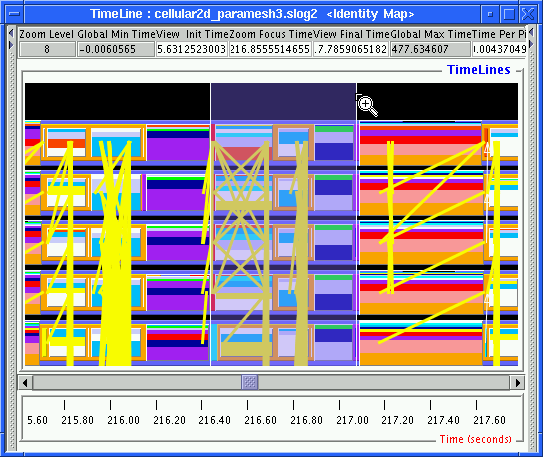
\includegraphics[%
  scale=0.6]{pic/timeline_preview_detail_0.png}


\caption{\label{fig:timeline_preview_detail_0} A typical zoom-out view of
preview states and arrows. The region that is marked by a pair of
white lines and the zoom-plus cursor is being zoomed in, i.e. enlarged,
in the next figure.}
\end{figure}


\noindent Each thick yellow line is a \emph{preview arrow} which represents
a collection of arrows between its 2 ending timelines. The start and
final timestamps of preview arrow are the extremes of all real arrows
amalgamated inside the preview object. Notice that the beginning or
ending timestamp of a preview arrow does not necessarily mean that
there is any arrow starting and ending at that times, it just indicates
that there are arrows starting or ending within these 2 times and
between the 2 marked timelines. The thickness of the preview arrow
denotes the number of real arrows represented by the preview object.
Because of the limitation on the available thickness that preview
arrow can have, the thickness of the preview object is set to equal
to the order of magnitude of the number of real objects amalgamated.
So same thickness in two different preview arrows does not mean that
they contain exactly the same number of real arrows, but does mean
that the numbers of real arrows contained in the preview objects are
within the same order of magnitude, i.e. within a constant multiplicative
factor as defined by PREVIEW\_ARROW\_LOG\_BASE in Preference window
shown in Figure \ref{fig:preference_pview_state} and in Table \ref{table:preference_zoomable_timeline}.
Different thickness in preview arrows indicates more than one multiple
of the constant factor difference in the number of real arrows between
the preview objects.

The rectangle that has horizontal strips of colors is \emph{preview
state}. The different colors inside a preview state represent the
various categories of real states that are amalgamated within the
time range of the preview state. Depending on the PREVIEW\_STATE\_DISPLAY
value selected in the pulldown menu at the top of left side Y-axis
label %
\footnote{In Preference window as shown in Figure \ref{fig:preference_pview_state}
and in Table \ref{table:preference_zoomable_timeline}, there is also
a PREVIEW\_STATE\_DISPLAY variable. The variable determines the initial
PREVIEW\_STATE\_DISPLAY used when Timeline window is first made visible.%
}, the distribution and the heights of the strips can be changed drastically.
One of the display options for preview state is \emph{CumulativeInclusionRatio}.
With this option, the strips are arranged in decreasing height order,
sort of like a small cumulative histogram. The tallest strip at the
bottom of the preview state corresponds to the category of states
that contribute the longest total duration in the specified time range
\emph{inclusively}, i.e. disregarding the nesting state order. This
visual representation aims to tell what state categories could be
within the span of the preview state and which state category contributes
the most statistically to the specified time range, so user can decide
where to zoom in to find out more details. In a sense, the preview
states provide a global coarse-grain summary of what is going on without
losing as much details as the preview found in older Jumpshot, i.e.
Jumpshot-3. Compared with Jumpshot-3's preview which has averaged
out the information about timeline IDs, the new preview states retain
the timeline ID information and that may lead to early detection of
load balancing problem before zooming in to see all the real states. 

\noindent %
\begin{figure}[!htbp]
\centering

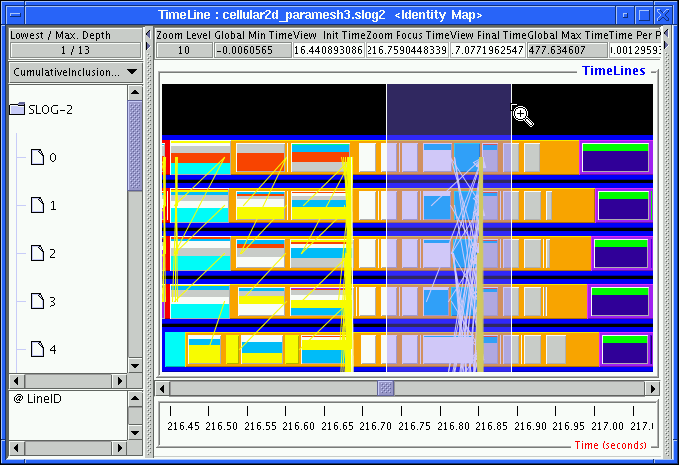
\includegraphics[%
  scale=0.6]{pic/timeline_preview_detail_1.png}


\caption{\label{fig:timeline_preview_detail_1} The next zoom-in view of Figure
\ref{fig:timeline_preview_detail_0}.}
\end{figure}


Figure \ref{fig:timeline_preview_detail_1} shows a more zoom-in view
of the region marked by the pair of white lines in Figure \ref{fig:timeline_preview_detail_0}.
In Figure \ref{fig:timeline_preview_detail_1}, some of the preview
arrows have disappeared and are replaced by real arrows, i.e. the
white arrows. Also, some of the stripped preview states have split
into several small preview states of identical color, i.e. the white
and gray states, to show more detailed distribution. Another important
feature of preview state becomes apparent in the figures: Preview
states are properly nested within real states. In the most expanded
Y-axis label view, preview state is always on top of other nested
states%
\footnote{Only in slog2 file that has multiple ViewMaps and where timelines
can be collapsed, i.e. AIX's UTE generated slog2 file, preview state
can be nested with other preview state in collapsed Y-axis label view.%
}, i.e. states that enclose the preview state are alway real states.
A good visual example is shown in Figure \ref{fig:timeline_preview_detail_1}
where all the white, turquoise and gray preview states%
\footnote{when a preview state contains only real states of one single category,
it may appear like a real state in the timeline canvas. The only sure
way to tell the difference is to bring up the Drawable Info Box by
right clicking on the state.%
} are sitting on top of the long orange and dark royal blue states.
This indicates that the white, turquoise and gray real states are
all nested inside the long running orange and dark royal blue states.

%
\begin{figure}[!htbp]
\centering

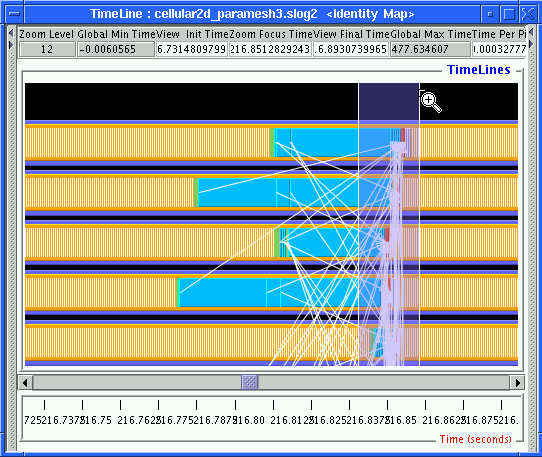
\includegraphics[%
  scale=0.6]{pic/timeline_preview_detail_2.png}


\caption{\label{fig:timeline_preview_detail_2} The next zoom-in view of Figure
\ref{fig:timeline_preview_detail_1}.}
\end{figure}


Figure \ref{fig:timeline_preview_detail_2} is the zoom-in view of
the region marked by the pair of white lines in Figure \ref{fig:timeline_preview_detail_1}.
Comparing these 2 figures, all the preview drawables have disappeared
and are replaced by real drawables. Each white preview state are replaced
by hundreds of white real states, the same is also true for the gray
preview states that sit to the right of the turquoise states%
\footnote{In order to speed up graphics performance of the display program,
an aggressive algorithm has been employed to eliminate drawing states
that are closely packed together within the nearest neighboring pixels.
Together with the fact that the number of pixels available is less
than the number of non-overlap states in the region, the number of
the real states may sometimes not appear as numerous as the Drawable
Info Box of preview state indicates. In that case, a further zoom
in will be needed to confirm the case as shown in Fig. \ref{fig:timeline_preview_detail_3}.%
}. The preview arrows are all replaced by the real arrows. It becomes
apparent that the white lines marked region in Figure \ref{fig:timeline_preview_detail_1}
provides a good description of what is going on in Figure \ref{fig:timeline_preview_detail_2}
but at the same time it reduces the number of drawables drawn on the
canvas by a factor of 100. Another way of seeing this benefit is to
find out the exact number of real drawables amalgamated by the preview
objects within the zoomed region. This can be achieved by right clicking
on the preview drawable and the result is shown in Figure \ref{fig:timeline_infobox_preview_state}.

%
\begin{figure}[!htbp]
\centering

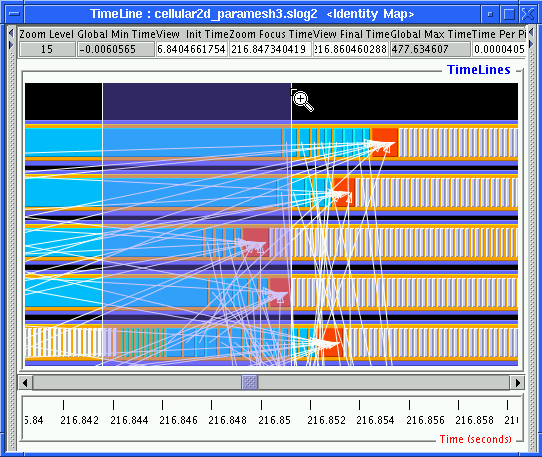
\includegraphics[%
  scale=0.6]{pic/timeline_preview_detail_3.png}


\caption{\label{fig:timeline_preview_detail_3} The next zoom-in view of Figure
\ref{fig:timeline_preview_detail_2}.}
\end{figure}


Further zooming into the white lines marked region in Figure \ref{fig:timeline_preview_detail_2}
enlarges the real drawables that are displayed in the figure. The
enlarged view is shown in Figure \ref{fig:timeline_preview_detail_3}.
The densely packed states and arrows become more distinguishable.
Another zooming in around the white lines marked region in Figure
\ref{fig:timeline_preview_detail_3} enlarges the real drawables into
easily separable objects as shown in Figure \ref{fig:timeline_preview_detail_4}.

%
\begin{figure}[h]
\centering

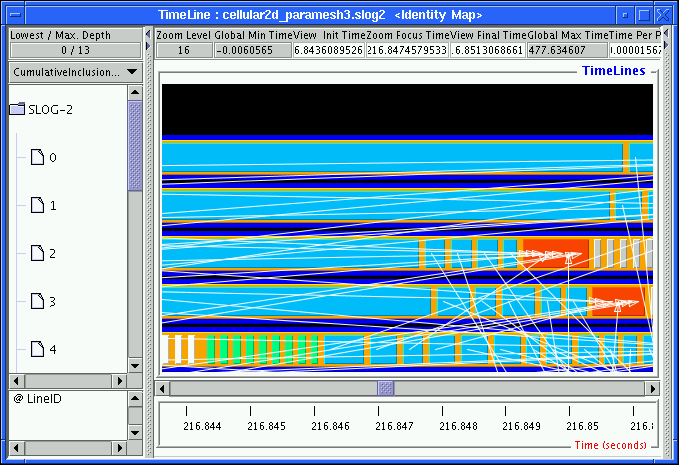
\includegraphics[%
  scale=0.6]{pic/timeline_preview_detail_4.png}


\caption{\label{fig:timeline_preview_detail_4} The next zoom-in view of Figure
\ref{fig:timeline_preview_detail_3}.}
\end{figure}


\clearpage



\subsection{Understanding the Preview State Display\label{sub:Preview-State-Display}}

So far only one of the representations of preview state, \emph{CumulativeInclusionRatio},
is used to illustrate the concept and representation of the preview
state. Jumpshot-4 actually uses several different representations
of preview state. All these representations are based on 2 ratios
stored in SLOG-2 file. They are called \emph{Inclusion Ratio} and
\emph{Exclusion Ratio.} Inclusion ratio is computed without taking
into account of the nesting order of the states. States which are
either nested inside or enclose other states contribute equally to
the inclusion ratio. The end result is that the sum of all inclusion
ratios from all state categories in a preview state could easily be
larger than 1. On the other hand, exclusion ratio is specifically
computed to exclude the overlap of the nested state from the enclosing
state. Therefore the sum of exclusion ratios of all state categories
in a preview state is guaranteed to be less than or equal to 1. 

The motivation of computing these 2 ratios is to satisfy two opposite
needs of preview state. If you are a MPI application developer and
you have put a lot of user-defined states in your SLOG-2 file through
either MPE or AIX's PCT utility, you most likely would be interested
in the profiling information of the user-defined states which enclose
MPI states and other user-defined states. In this case, inclusion
ratio will be very useful. Because inclusion ratios of user-defined
states usually dominate all state inclusion ratios, including those
of MPI states. Therefore, the inclusion ratio highlights the outermost
enclosing states even at high preview level. On the other hand, if
you are a MPI implementor or are interested in the low level MPI networking
overhead, you are most likely interested in the profiling information
of MPI and its internal calls. Exclusion ratio will come in handy.
Exclusion ratios for the innermost nested states, i.e. MPI states,
tend to dominate all state exclusion ratios. So the exclusion ratio
highlights the innermost nested states at very high preview level.

%
\begin{figure}[!htbp]
\centering
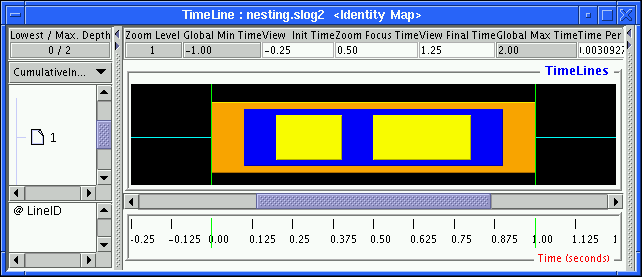
\includegraphics[%
  scale=0.5]{pic/timeline_nesting_detail.png}


\caption{\label{fig:timeline_nesting_detail}A zoomed in view of some nested
states where the duration of the orange state is 1.0 sec. The duration
of the navy blue state is 0.8 sec. The sum of durations for the 2
yellow states is 0.5 sec.}
\end{figure}


Figure \ref{fig:timeline_nesting_detail} shows a typical zoomed in
view of some nested states. In this view, the yellow states are deeply
nested in the navy blue state which is in turns nested in the orange
state. The pair of green lines mark the region where a preview state
is being created for.

%
\begin{table}[!htbp]
\begin{longtable}{|c|c|c|c|c|}
\hline 
Icon&
Description&
Duration&
Inclusion Ratio&
Exclusion Ratio\tabularnewline
\hline
\hline 
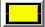
\includegraphics[%
  scale=0.8]{pic/timeline_nesting_legend_innermost.png}&
Innermost Nested State&
0.5 sec&
50\%&
50\%\tabularnewline
\hline 
\multicolumn{1}{|c|}{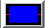
\includegraphics[%
  scale=0.8]{pic/timeline_nesting_legend_middle.png}}&
Intermediate Nested State&
0.8 sec&
80\%&
30\%\tabularnewline
\hline 
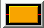
\includegraphics[%
  scale=0.8]{pic/timeline_nesting_legend_outermost.png}&
Outermost Enclosing State&
1.0 sec&
100\%&
20\%\tabularnewline
\hline
\end{longtable}


\caption{\label{table:legend_nesting_detail}The breakdown of real states'
contribution to a preview state of duration 1.0 sec as it is marked
by a pair of green lines in Figure \ref{fig:timeline_nesting_detail}.}
\end{table}


The inclusion and exclusion ratios are computed for the region marked
by the pair of green lines and are shown in Table \ref{table:legend_nesting_detail}.
The table shows that the most dominant state among all inclusion ratios
is the orange outermost state, but the most dominate state among all
exclusion ratios is the yellow innermost state which is the least
dominant state in inclusion ratios. One obvious observation is that
the inclusion and exclusion ratios of the innermost state category
are the same.

%
\begin{figure}[!htbp]
\centering
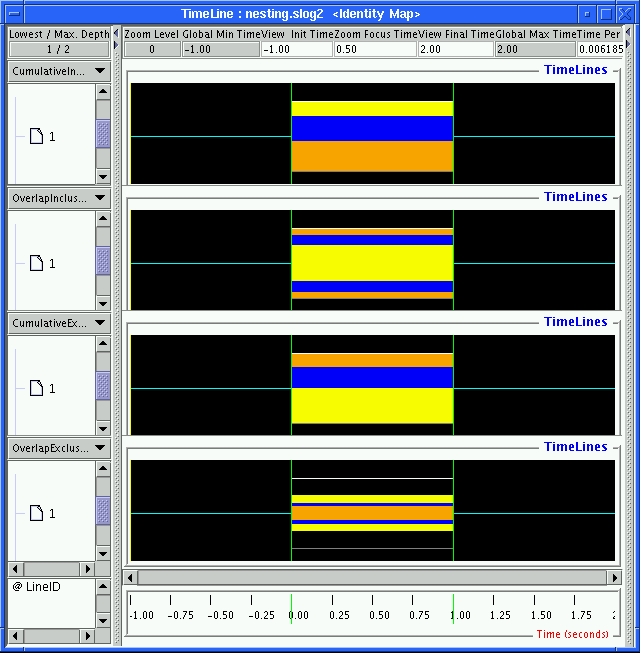
\includegraphics[%
  scale=0.5]{pic/timeline_nesting_preview_all.png}


\caption{\label{fig:timeline_nesting_preview_all} Different preview state
displays of the zoomed in view of the Figure \ref{fig:timeline_nesting_detail}.
Starting from the top, the first one is \emph{CumulativeInclusionRatio}
view, the second one is \emph{OverlapInclusionRatio} view, the third
one is \emph{CumulativeExclusionRatio} view, and the last one is \emph{OverlapExclusionRatio}
view.}
\end{figure}


With data computed in Table \ref{table:legend_nesting_detail}, various
different preview displays can be drawn and are shown in Figure \ref{fig:timeline_nesting_preview_all}.
All colored strips inside the preview state will be drawn proportional
to the height of the preview state. For instance, if the ratio of
the category for the strip is 0.9, the corresponding colored strip
will occupy 90\% of the preview state's height. The statement is true
for all preview state display except \emph{CumulativeInclusionRatio}
which could have its total sum of ratios in exceed of 1.0 especially
when the slog2 file is highly nested. First consider the \emph{CumulativeInclusionRatio}
and \emph{CumulativeExclusionRatio} views, i.e the first and the third
ones from the top in the figure. Notice that yellow state is least
important in the top \emph{CumulativeInclusionRatio} view, but becomes
most significant in the third \emph{CumulativeExclusionRatio} view.
Since the sum of all inclusion ratios is larger than 1, in this case,
the sum is 2.3, the \emph{CumulativeInclusionRatio} view reweights
all ratios to fill up the preview box. Strictly speaking \emph{CumulativeInclusionRatio}
view cannot be used to compare different preview states because of
the arbitrary rescaling%
\footnote{Most of times, neighoring preview states in \emph{CumulativeInclusionRatio}
view has similar total sum of inclusion ratios. Because of this fact,
one can compare adjacent preview states. But bear in mind that the
total sum of inclusion ratios between nearby preview states can change
drastically without any visual indication. When in doubt, right click
on the preview state to get Drawable Info Box to confirm the ratios.%
}. If one is interested in the comparison of inclusion ratios across
different preview states, \emph{OverlapInclusionRatio} view can be
used instead. \emph{OverlapInclusionRatio} view draws all inclusion
ratios proportional to the height of the preview state but in an overlapping
way, i.e. draw them in decreasing inclusion ratios order and stack
one on top of the other, sort of like nested state. The overlap view
of exclusion ratios is \emph{OverlapExclusionRatio} view which is
shown at the bottom of Figure \ref{fig:timeline_nesting_preview_all}.
\emph{OverlapExclusionRatio} view draws exclusion ratios exactly the
same way as \emph{OverlapInclusionRatio}. In general, overlap view
cannot fill up the full height of the preview state. This is apparent
in \emph{OverlapExclusionRatio} view in \ref{fig:timeline_nesting_preview_all}
where the white bordered box indicates the full height of the preview
state. The white bordered box is necessary in comparing the ratios
across different preview states with respect to the preview states'
duration. However, the white bordered box can sometimes be confusing,
because whatever in the back of the preview state can show through
the empty space within the white bordered box. In that case, the bordered
box can be turned off by selecting \emph{Empty} in PREVIEW\_STATE\_BORDER
in Preference window. 

For the sake of comparison and continuity with our preview discussion,
the \emph{CumulativeExclusionRatio} view of Figures \ref{fig:timeline_preview_detail_0}
and \ref{fig:timeline_preview_detail_1} are shown in Figures \ref{fig:timeline_preview_detail_0_excl}
and \ref{fig:timeline_preview_detail_1_excl} respectively. The \emph{CumulativeExclusionRatio}
view does provide an extra dimension of information when compared
to its inclusion ratio counterpart at the expense of being a bit more
complicated to digest visually.

%
\begin{figure}[!htbp]
\centering
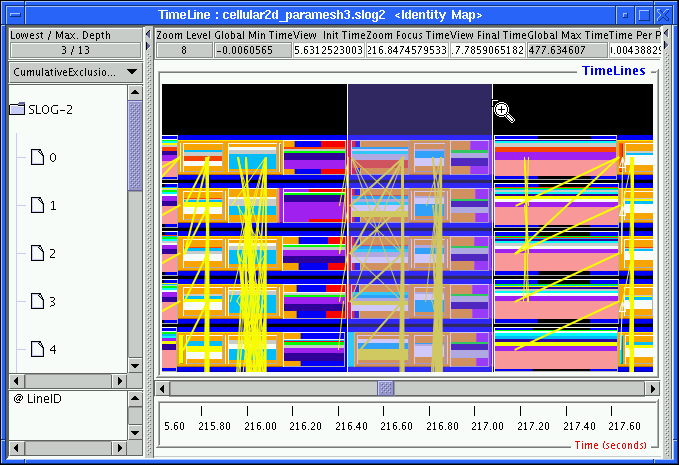
\includegraphics[%
  scale=0.6]{pic/timeline_preview_detail_0_excl.png}


\caption{\label{fig:timeline_preview_detail_0_excl} The \emph{CumulativeExclusionRatio}
view of Figure \ref{fig:timeline_preview_detail_0}.}
\end{figure}


%
\begin{figure}[!htbp]
\centering
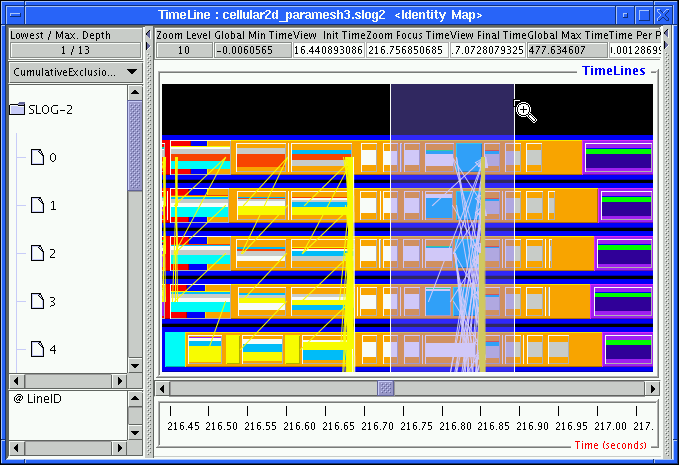
\includegraphics[%
  scale=0.6]{pic/timeline_preview_detail_1_excl.png}


\caption{\label{fig:timeline_preview_detail_1_excl}The \emph{CumulativeExclusionRatio}
view of Figure \ref{fig:timeline_preview_detail_1}. Also, a zoom-in
shot of Figure \ref{fig:timeline_preview_detail_0_excl}.}
\end{figure}


\clearpage



\chapter{Graphical User Interface}


\section{Main Window}

%
\begin{figure}[!htbp]
\centering
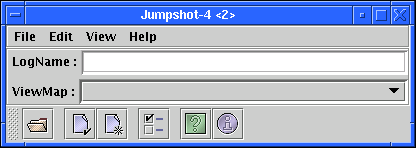
\includegraphics[%
  scale=0.6]{pic/main.png}


\caption{\label{fig:main} The main control window of Jumpshot-4.}
\end{figure}


The first window that pops up when invoking Jumpshot-4 is called Main
window as shown in Figure \ref{fig:main}. The buttons shown in toolbar
are shortcuts to the sub menu items in the top menubar. The function
of each of these buttons is listed in the Table \ref{table:main_toolbar}.
There are 2 text fields that display crucial information about the
logfile being processed. The text field which is titled \emph{LogName}
displays the pathname of the logfile being processed. The pulldown
menu which is titled \emph{ViewMap} lists all the available ViewMaps
in the SLOG-2 file. Currently, both CLOG%
\footnote{a low-overhead native trace format from MPE.%
} and RLOG%
\footnote{an internal MPICH2 profiling format%
} converted SLOG-2 file contains one ViewMaps, it is called the Identity
Map. Only IBM's UTE trace converted SLOG-2 file contains multiple
ViewMaps.

%
\begin{table}[!htbp]
\begin{longtable}{|c|c|c|}
\hline 
Icon&
Description&
Function\tabularnewline
\hline
\hline 

\includegraphics[%
  scale=0.8]{pic/gif2png/Open24.png}&
File Selection &
display a File Chooser dialog to select logfile to be processed\tabularnewline
\hline 

\includegraphics[%
  scale=0.8]{pic/gif2png/Convert24.png}&
Logfile Conversion&
invoke the Logfile Convertor to convert non-slog2 file to slog2 format\tabularnewline
\hline 

\includegraphics[%
  scale=0.8]{pic/gif2png/Properties24.png}&
Show Legend Window&
display the Legend window of the selected logfile if it is hidden\tabularnewline
\hline 

\includegraphics[%
  scale=0.8]{pic/gif2png/New24.png}&
Show Timeline Window&
display the Timeline window of the selected logfile if it is hidden\tabularnewline
\hline 

\includegraphics[%
  scale=0.8]{pic/gif2png/Preferences24.png}&
Edit Preferences&
display the Preference window that adjusts Jumpshot's properties\tabularnewline
\hline 

\includegraphics[%
  scale=0.8]{pic/gif2png/Help24.png}&
Show User's Manual&
show the User's Manual of this program\tabularnewline
\hline

\includegraphics[%
  scale=0.8]{pic/gif2png/Information24.png}&
Show FAQs&
show the FAQs of this program\tabularnewline
\hline
\end{longtable}


\caption{\label{table:main_toolbar} Functions of the toolbar buttons}
\end{table}



\section{Logfile Convertor Window}

%
\begin{figure}[!htbp]
\centering
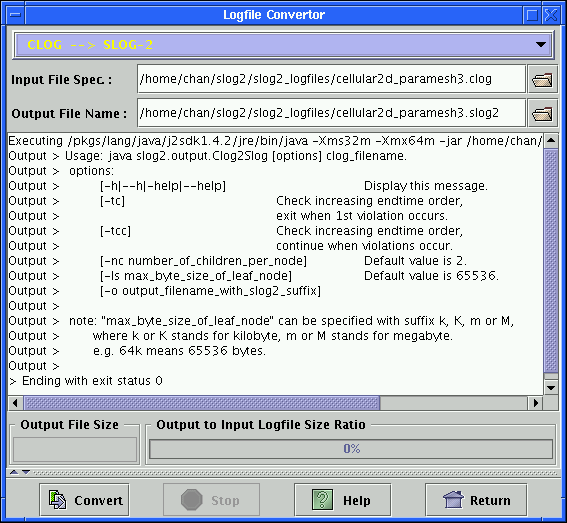
\includegraphics[%
  scale=0.5]{pic/convertor_init.png}


\caption{\label{fig:convertor_init}The Logfile Convertor window that allows
conversion of supported trace file format to SLOG-2 format.}
\end{figure}


If a non-slog2 file is selected in the Main window, the Logfile Convertor
as shown in Figure \ref{fig:convertor_init} will be invoked to prompt
user to convert the file to SLOG-2 format readable by this viewer.
There are currently 3 supported convertors: \emph{CLOG} --\textgreater{}
\emph{SLOG-2}, \emph{RLOG} --\textgreater{} \emph{SLOG-2} and \emph{UTE}
--\textgreater{} \emph{SLOG-2.} Convertor is generally selected based
on the input file's file extension. In the case that wrong file convertor
is selected, user can correct it through the pale blue pulldown menu
located at the top of the window. The Logfile Convertor window can
also be invoked by directly clicking on the Logfile Conversion button
shown in the Table \ref{table:main_toolbar}. The text field of the
Output File Name usually displays the default slog2 filename recommended
by the convertor based on the text field in the Input File Specification.
If the text field does not display the default name as expected, hitting
return key in the Input File Specification field will force the update
of the Output File Name field with the default name. There are 4 major
functions of the Logfile convertor and each of them is associated
with a button in the lower panel of the window. They are listed in
the Table \ref{table:convertor_buttons}.

%
\begin{table}[!htbp]
\begin{longtable}{|c|c|c|}
\hline 
Icon&
Description&
Function\tabularnewline
\hline
\hline 

\includegraphics[%
  scale=0.8]{pic/gif2png/Convert24.png}&
Start Conversion&
Start the logfile conversion of the selected convertor\tabularnewline
\hline 

\includegraphics[%
  scale=0.8]{pic/gif2png/Stop24.png}&
Stop Conversion&
Stop the ongoing logfile conversion of the selected convertor\tabularnewline
\hline 

\includegraphics[%
  scale=0.8]{pic/gif2png/Help24.png}&
Usage of Convertor&
Print the usage information of the selected convertor\tabularnewline
\hline 

\includegraphics[%
  scale=0.8]{pic/gif2png/Home24.png}&
Return Home&
Return to the previous component that spawns the Logfile Convertor\tabularnewline
\hline
\end{longtable}


\caption{\label{table:convertor_buttons}Functions of the major functions
in the Logfile Convertor window.}
\end{table}


Since the Logfile Convertor launches a separate java process to do
the logfile conversion, it requires certain parameters to launch the
process correctly. All the parameters that are needed by any logfile
convertor are supplied through a panel hidden by a splitter in the
convertor window. The splitter has a divider which can be lifted up
to display all the parameters used to launch the java process as in
the Figure \ref{table:convertor_buttons}. In the rare occasion that
the default parameters are not correct, the text fields can be modified
to reflect the situation. 

%
\begin{figure}[!htbp]
\centering
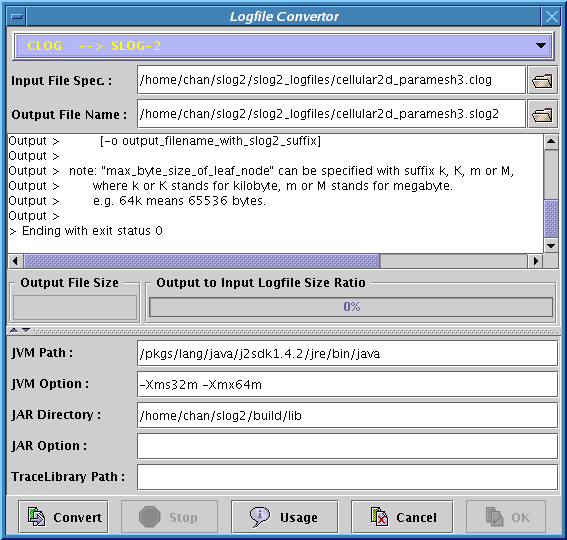
\includegraphics[%
  scale=0.5]{pic/convertor_parameters.png}


\caption{\label{fig:convertor_parameters}The hidden parameters panel of the
Logfile Convertor.}
\end{figure}


The standard output and error streams of the process are being piped
to the text area located in the middle of the window as the process
is running. The Output File Size field displays the current size of
the slog2 file as it is being generated, also the progress bar will
be incremented to show the current ratio of the output to input file
size as in the Figure \ref{fig:convertor_progress}. If the logfile
conversion fails, the error message will be printed in the text area
for diagnosis or bug report.

%
\begin{figure}[!htbp]
\centering
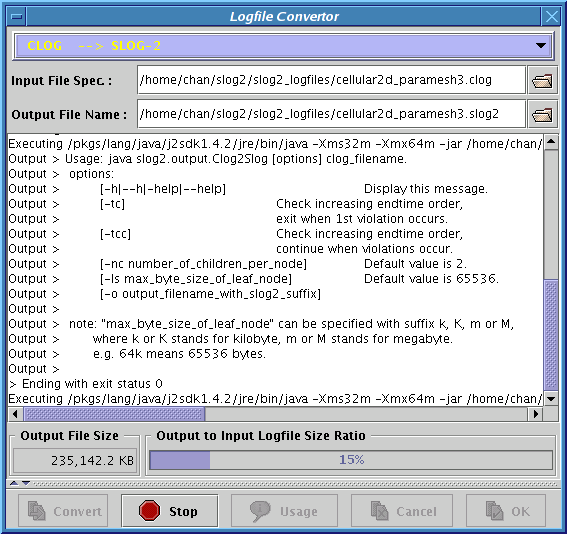
\includegraphics[%
  scale=0.5]{/home/chan/slog2/slog2sdk_2b/doc/jumpshot-4/tex/pic/convertor_progress.png}


\caption{\label{fig:convertor_progress} Logfile conversion in progress.}
\end{figure}


\clearpage



\section{Legend Window}

As soon as a SLOG-2 file is selected in Main window and ready for
visualization, the Legend window like the one shown in Figure \ref{fig:legend_popup}
will be displayed. All the features that are going to be discussed
in the Legend window affects both the Timeline and Histogram windows.

%
\begin{figure}[!htbp]
\centering
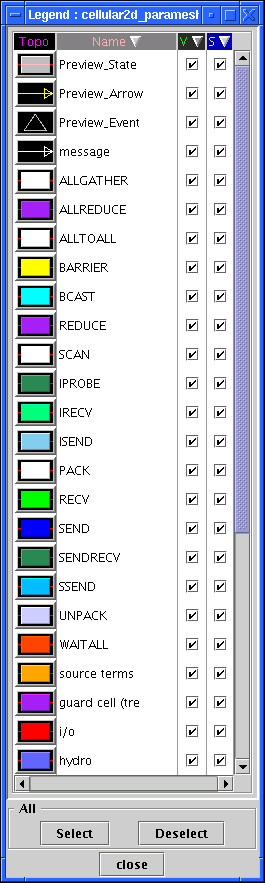
\includegraphics[%
  scale=0.6]{pic/legend_popup.png}


\caption{\label{fig:legend_popup} A typical Legend window when slog2 file
is first loaded into Jumpshot-4.}
\end{figure}


The Legend window contains mainly a 4-columns legend table. The 4
columns are labeled as \emph{Topo, Name, V} and \emph{S} as in Table
\ref{table:legend_column_ops}.

%
\begin{table}[!htbp]
\begin{longtable}{|c|c|>{\centering}p{2in}|m{2in}|}
\hline 
\multicolumn{1}{|c|}{Icon}&
Description&
Left Mouse Click on Column Cell&
Right Mouse Click on Column Cell or Left Mouse Click on Column Title\tabularnewline
\hline
\hline 

\includegraphics[%
  scale=0.8]{pic/legend_topo.png}&
Topology&
Pick new Color (Figure \ref{fig:legend_color_chooser})&
None\tabularnewline
\hline 

\includegraphics[%
  scale=0.8]{pic/legend_name.png}&
Name&
Edit Name&
Sort Order menu (Figure \ref{fig:legend_sort_order})\tabularnewline
\hline 

\includegraphics[%
  scale=0.8]{pic/legend_v.png}&
Visibility&
Check or Uncheck&
Checkbox Operations Menu (Figure \ref{fig:legend_checkbox_ops})\tabularnewline
\hline 

\includegraphics[%
  scale=0.8]{pic/legend_s.png}&
Searchability&
Check or Uncheck&
Checkbox Operations Menu (Figure \ref{fig:legend_checkbox_ops})\tabularnewline
\hline
\end{longtable}


\caption{\label{table:legend_column_ops} Operations on the Legend window's
columns.}
\end{table}


Table \ref{table:legend_column_ops} also lists out all defined mouse
operations that are provided in each column. The operations are (1)
left mouse clicking on the column title icon and on the column cell
as well as (2) right mouse clicking in any column cell. 

%
\begin{figure}[!htbp]
\centering
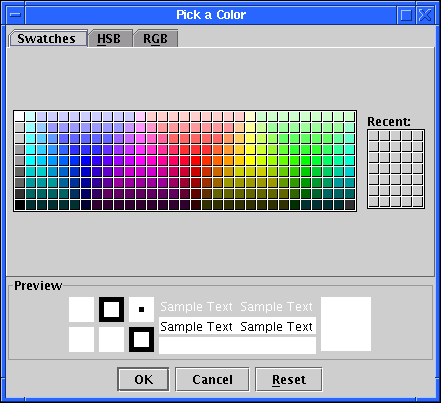
\includegraphics[%
  scale=0.6]{pic/legend_color_chooser.png}


\caption{\label{fig:legend_color_chooser} Color Chooser Dialog for column
Category Topology}
\end{figure}


Figure \ref{fig:legend_color_chooser} is the Color Chooser dialog
that will pop up when one of the icon buttons in column Topo is pressed.
The color editor provides 3 different ways of choosing a new color.
After selecting a new color from the dialog, the new color will be
used to update the icon button. The update won't be carried out in
the timeline canvas automatically, explicit screen redraw is needed.

%
\begin{figure}[!htbp]
\centering
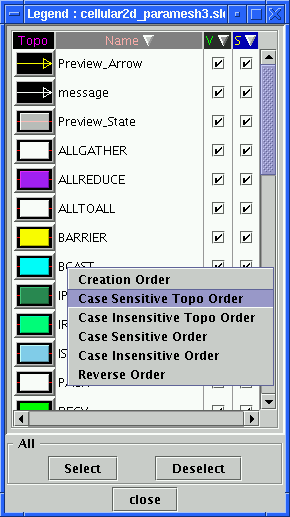
\includegraphics[%
  scale=0.6]{pic/legend_sort_menu.png}


\caption{\label{fig:legend_sort_order} Sort Order operation menu for the
column Category Name in the Legend window.}
\end{figure}


Figure \ref{fig:legend_sort_order} shows the popup dialog box either
when the title icon of column Name is pressed or when right mouse
button is clicked somewhere in the column. There are altogether 6
different sort orders. The first 4 orderings are various combination
of alphabetical and case sensitive order, e.g. \emph{z...a Z...A}
refers reverse case sensitive alphabetical ordering. The second last
order in the list is called \emph{Creation Order} which refers to
the order in which categories are stored in slog2 file when they are
being created. The 4 alphabetical ordering has 2 hidden sort orders.
One is called \emph{Preview Order} which puts the preview drawable
category before all the real drawable categories of the same topology.
The other is \emph{Topo Order} which refers to topological ordering,
i.e arrow is ahead of state. The preview and topo sort orders can
be turned on or off through the Preference window as shown in Table
\ref{table:preference_legend}. 

%
\begin{table}[!htbp]
\centering
\begin{longtable}{|c|c|}
\hline 
Ordering&
Description\tabularnewline
\hline
\hline 
\emph{A...Z a...z}&
case sensitive alphabetical ordering\tabularnewline
\hline 
\emph{z...a Z...A}&
reverse case sensitive alphabetical ordering\tabularnewline
\hline 
\emph{Aa...Zz}&
case insensitive alphabetical ordering\tabularnewline
\hline 
\emph{zZ...aA}&
reverse case insensitive alphabetical ordering\tabularnewline
\hline 
Creation&
category storage ordering in the slog2 file\tabularnewline
\hline 
Reverse Creation&
reverse of Creation order\tabularnewline
\hline
\end{longtable}


\caption{\label{table:legend_sort_orders}The Description of the Sort Order
operation menu in the Legend window.}
\end{table}


%
\begin{figure}[!htbp]
\centering
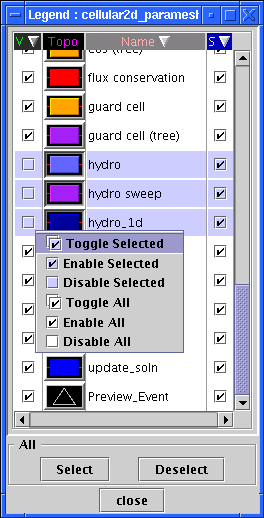
\includegraphics[%
  scale=0.6]{pic/legend_checkbox_menu.png}


\caption{\label{fig:legend_checkbox_ops} Checkbox Operation menu for column
Category Visibility and Searchability }
\end{figure}


Figure \ref{fig:legend_checkbox_ops} shows a popup dialog box when
the title icon of column V (Visibility) or S (Searchability) is pressed
or when right mouse button is clicked somewhere in either columns.
The rule of selection in the legend table follows the standard practice
of other graphical user interfaces as in the Table \ref{table:selection_rules}.
Together with this standard selection rules, the operations provided
in checkbox operation menu allow easy enabling and disabling of visibility
as well as searchability checkboxes. With the help of continuous selection
of the category rows in the legend table and various sort ordering
available, users can easily make a huge number of categories disappear
in the Timeline or Histogram window. For instance, in CLOG converted
SLOG-2 file where upper case name always refers to MPI names, the
case sensitive alphabetical ordering allows all MPI names to be put
before all user-defined categories. With continuous mouse selection,
user can easily toggle the visibility of user-defined states in the
Timeline or Histogram window. Also, every element in the column Name
is editable. This allows user to correct undesirable category names
set during logfile creation or even facilitate sorting of the names
for selection purposes.

%
\begin{table}[!htbp]
\begin{longtable}{|c|>{\centering}m{4in}|}
\hline 
Left Mouse Operation&
Action\tabularnewline
\hline
\hline 
\noun{Click}&
\emph{Click} on an object deselects any existing selection and selects
the object.\tabularnewline
\hline 
\noun{Control-Click}&
\emph{Control-click} on an object toggles its selection without affecting
the selection of any other objects\tabularnewline
\hline 
\noun{Shift-Click}&
\emph{Shift-click} on an object extends the selection from the most
recently selected object to the current object.\tabularnewline
\hline 
\noun{Dragging }&
\emph{Dragging} (that is, moving the mouse while holding down left
mouse button) through a range of \noun{text} deselects any existing
selection and selects the range of text.\tabularnewline
\hline
\end{longtable}


\caption{\label{table:selection_rules} Standard Selection Rules.}
\end{table}


\noun{NOTE:} Any changes done in the Legend window that alters the
appearance of drawables won't be automatically updated in the timeline
canvas until the CanvasReDraw button in the Timeline window is pressed.


\section{Timeline \emph{Zoomable} Window}

%
\begin{figure}[!htbp]
\centering
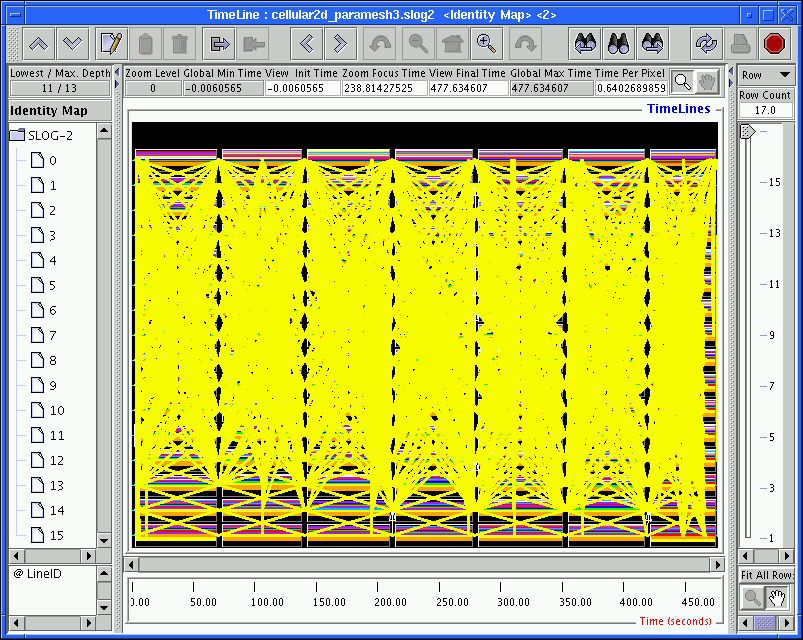
\includegraphics[%
  scale=0.5]{pic/timeline_popup.png}


\caption{\label{fig:timeline_popup} The initial display of the Timeline window
of a 514 MB 16 processes slog2 file with default preview resolution.}
\end{figure}


Most of the advanced features in the SLOG-2 viewer are provided through
\emph{}the \emph{Zoomable} window. There are two zoomable windows
in Jumpshot-4: Timeline and Histogram windows. Figure \ref{fig:timeline_popup}
is the initial display of the Timeline window of a half gigabyte 16
timelines slog2 file. Zoomable window consists of several concealable
and removable components. In the center of the window, it is the \emph{zoomable
and scrollable canvas}. For Timeline window, the center canvas is
called \emph{timeline canvas}. Directly on top of the zoomable canvas
is the \emph{time display panel}. On top of the display panel, there
is the removable \emph{toolbar}. To the left of the canvas is the
concealable \emph{Y-axis label panel}. To the right of the canvas
is the concealable \emph{row adjustment panel}. At the bottom of the
canvas is the \emph{time ruler canvas}. Both Y-axis label and the
row adjustment panels can be put out of sight by clicking the tabs
in the dividers or dragging the dividers to the side of the window.
The top toolbar can be dragged out of the window or be repositioned
in the other 3 sides of the window. A bare minimal zoomable window
can be obtained by the removal of toolbar and the hiding of the left
and right panels. An almost bare minimal Timeline window looks like
the one shown in Figure \ref{fig:timeline_preview_detail_0}. 


\subsection{Zoomable and Scrollable Canvas\label{sub:Zoomable-and-Scrollable}}

When viewing a big slog2 file like the one shown in Figure \ref{fig:timeline_popup},
the whole timeline canvas is filled up with preview drawables. Though
it provides a reasonable description at high level%
\footnote{Reasonable description here means that user can still get a vague
sense of where the long and/or frequent drawables are .%
}, it is pretty obscure to know the details. Hence, a well-designed
zoomable and scrollable user interface (ZSUI) of the timeline canvas
becomes an absolute necessity to facilitate the location of events
of interest. The ZSUI of the timeline canvas includes many parts and
operations. But the most handy ones are \emph{dragged zoom}, \emph{grasp
and scroll} and \emph{instant zoom in and out.} All these features
are supported by the \emph{Zoomable and Scrollable canvas}. There
are 2 such canvases in the Timeline window. They are \emph{Timeline
Canvas} and \emph{Time Ruler Canvas}. In these canvases, left mouse
clicking can be alternated in 2 different modes by a pair of toggled
buttons as shown in Figures \ref{fig:mouse_zoom_mode} and \ref{fig:mouse_hand_mode}.
They are called \emph{Zoom} and \emph{Hand} modes. Each canvas in
the Timeline window has its own set of toggled buttons that determine
its left mouse click behavior. The timeline canvas's toggled buttons
are located above the canvas and sit at the end of the time display
panel. The time ruler's toggled buttons are located at the bottom
of row adjustment panel, i.e. sit right next to the end of the ruler.
By default, the timeline canvas is in zoom mode and the time ruler
canvas is in hand mode, so user can do zooming when the cursor is
in the timeline canvas and can scroll easily by simply moving the
cursor over the ruler canvas. Also, the scrolling can be done by simply
dragging on scrollbar's knob, clicking the end buttons and in the
space between the knob and scrollbar's end buttons.

%
\begin{figure}[!htbp]
\centering

\includegraphics{pic/mouse_zoom_mode.png}


\caption{\label{fig:mouse_zoom_mode} Canvas's left mouse click is in zoom
mode.}
\end{figure}


%
\begin{figure}[!htbp]
\centering

\includegraphics{pic/mouse_hand_mode.png}


\caption{\label{fig:mouse_hand_mode} Canvas's left mouse click is in hand
mode.}
\end{figure}



\subsubsection{Dragged Zoom}

%
\begin{figure}[!htbp]
\centering

\includegraphics{pic/gif2png/ZoomPlusUpLeft25.png}


\caption{\label{fig:zoom_plus_cursor} Zoom-plus cursor that indicates the
left mouse clicking is ready for zooming in.}
\end{figure}


\emph{Dragged zoom} is active only when the left mouse click is in
zoom mode, i.e. when the the magnifying glass button is pressed in
the toggled buttons as in Figure \ref{fig:mouse_zoom_mode}. In zoom
mode, the cursor within the canvas will appear like a magnifying glass
with plus sign in the center as in Figure \ref{fig:zoom_plus_cursor}.
It is called zoom-plus cursor. The dragged zoom operation is initialized
by pressing the left mouse button at the beginning of the zoom-in
region, a white line will then appear. As soon as dragging is detected,
another white line will appear to mark the current ending of the zoom-in
region. The region that is marked by pair of white lines is lightly
shaded as shown in Figure \ref{fig:timeline_preview_detail_3}. The
process can be canceled anytime by hitting the ESC key during dragging.
Once the left mouse button is released, zooming will be carried out
and the Timeline window will then be updated as in Figure \ref{fig:timeline_preview_detail_4}.
The time display panel is updated with the latest time related information
of the zoom-in region. Notice that the zooming as well as scrolling
can be achieved by explicitly editing the text fields in the time
display panel.


\subsubsection{Instant Zoom}

%
\begin{figure}[!htbp]
\centering

\includegraphics{pic/gif2png/ZoomMinusUpLeft25.png}


\caption{\label{fig:zoom_minus_cursor} Zoom-minus cursor that indicates the
left mouse clicking is ready for zooming out.}
\end{figure}


While the canvas is still in zoom mode, \emph{instant zoom} is enabled
by default. Instant zoom allows zooming in at the point of left mouse
clicking by a factor of 1/2, i.e. the region centered at the point
of left clicking will be magnified by a factor or 2. Also, the \emph{Zoom
Focus Time} in the time display panel will be updated with the time
where left clicking on the canvas is detected. In the process, the
cursor remain\emph{s} zoom-plus cursor. \emph{Shift-click}, on the
other hand, will do the opposite. While holding down Shift key, the
cursor will be changed to a zoom-minus cursor as in Figure \ref{fig:zoom_minus_cursor}
to indicate zooming out is the action associated with left clicking.
The zoom factor is 2 in this case.


\subsubsection{Grasp and Scroll}

%
\begin{figure}[!htbp]
\centering

\includegraphics{pic/gif2png/HandOpenUpLeft25.png}


\caption{\label{fig:hand_open_cursor} Open hand cursor indicates that left
mouse clicking is ready to grasp and scroll.}
\end{figure}


%
\begin{figure}[!htbp]
\centering

\includegraphics{pic/gif2png/HandCloseUpLeft25.png}


\caption{\label{fig:hand_close_cursor} Close hand cursor indicates that left
mouse clicking is scrolling.}
\end{figure}


\emph{Grasp and Scroll} is active only when the left mouse click is
in hand mode, i.e. when the open hand button is pressed as in Figure
\ref{fig:mouse_hand_mode}. The cursor in hand mode is an open hand
as in Figure \ref{fig:hand_open_cursor}. As soon as left mouse button
is pressed down, the cursor turns to a close hand as in Figure \ref{fig:hand_close_cursor}.
It indicates the canvas will move in the same direction that the cursor
moves as long as the left mouse button remain pressed. The grasp and
scroll mode in time ruler canvas can only move horizontally, but the
grasp and scroll mode in timeline canvas allows movement in both vertical
and horizontal axes. 


\subsubsection{Information Dialog Box}

Jumpshot-4 wouldn't be complete if it cannot provide a way to tell
user what exactly are being displayed. It is particularly important
when there are many preview drawables. Following standard user interface
practice, Jumpshot-4 uses \emph{right mouse clicking} as an interface
for user to tell Jumpshot-4 what object that more information is needed.
In general, anywhere on the canvas, both timeline and time ruler canvases,
can be inquired with right mouse clicks. Information dialog box will
pop up accordingly to tell user more about object that is being clicked.
There are 3 different types of information dialogs: Drawable Info
Box, Duration Info Box and Time Info Box. All these info boxes remain
in memory as long as they are not closed even if the canvas has been
scrolled or zoomed. One of the usages of the info boxes is to serve
as time markers in between zooming and scrolling.


\paragraph{Drawable Info Box}

Drawable Info Box is a popup dialog box that provides detailed information
about the drawable object that is being clicked. There are 2 different
kind of Drawable Info Box, one for preview drawable, one for real
drawable. 


\subparagraph{Drawable Info Box for Preview Drawable}

%
\begin{figure}[!htbp]
\centering

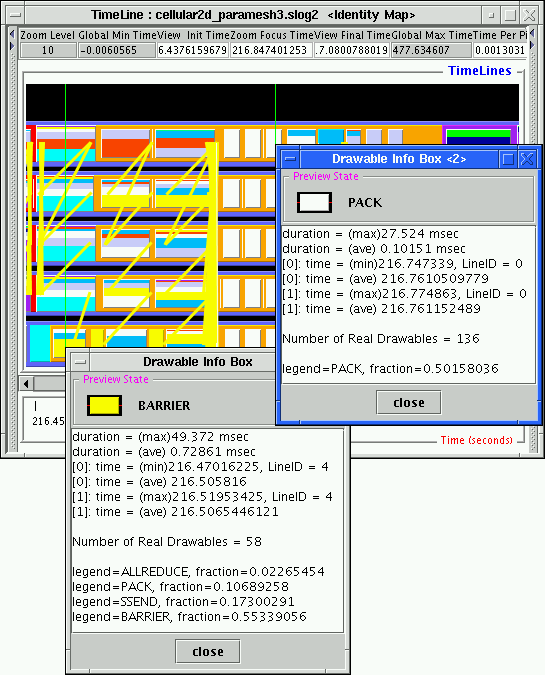
\includegraphics[%
  scale=0.6]{pic/timeline_infobox_preview_state.png}


\caption{\label{fig:timeline_infobox_preview_state} Drawable Info Box for
Preview State}
\end{figure}


Right mouse clicking on 2 of the preview states in the timeline canvas
shown in Figure \ref{fig:timeline_preview_detail_1_excl} will pop
up 2 Drawable Info Boxes for the preview states. They are displayed
in Figure \ref{fig:timeline_infobox_preview_state}. The popup Info
Box's upper left hand corner will be positioned at exactly where right
mouse click is detected and a green line marker will appear on the
canvas to indicate what time has been clicked in case the dialog box
is moved from its original popup location. In order to best illustrate
what information is presented by the Drawable Info Box, let's take
the highlighted Drawable Info Box in Figure \ref{fig:timeline_infobox_preview_state}
as an example. The Drawable Info Box for preview state contains a
pink label {}``Preview State'', and the icon inside the dialog box
shows the color and shape of the drawable. Below the icon, there is
a big text area that prints all the detailed statistical information
about this preview state. There are 6 timestamps in the text area:
maximum duration, minimum starttime, maximum endtime, average duration,
average starttime and average endtime. Here {}``{[}0{]}'' refers
to starting point, and {}``{[}1{]}'' refers to the ending point.
The 3 {}``average'' timestamps are averaged over all the real drawables
represented by this preview drawable. Besides timestamps, the info
box also tells {}``Number of Real Drawables'' represented by the
preview object. In this case, 136 real states are amalgamated by the
pure white preview state. Also, the text area lists all the categories
of real drawables amalgamated and their ratios of the total duration
of all real drawables to the duration of the preview states. In this
case, there is only 1 category of real states in this preview state,
so all 136 states are all PACKs. The sum of the durations of all PACKs
is about half of the duration of the preview state as it is indicated
by {}``ratio=0.5021433''. 

Another Drawable Info Box which is shown in Figure \ref{fig:timeline_infobox_preview_state}
has its upper left-hand pointed at a preview state that has 4 different
strips of colors: yellow, royal blue, white and purple. Right mouse
clicking at the yellow strip pops up a Drawable Info Box with a yellow
state icon with label BARRIER. As shown in the figure, this preview
state amalgamated 4 different categories of real states: ALLREDUCE,
PACK, SSEND, and BARRIER, and the statistically most significant one
is BARRIER. It proportionally and exclusively occupies 55\% of the
length of the preview state. Hence BARRIER strip has the tallest height
among all the color strips shown in the preview state. Clicking on
the different color strip in the same preview state will pop up a
Drawable Info Box with a different labeled icon, but the content of
the text area remains the same. In general, not every category listed
in the text area is visible in the preview state display. Out of the
4 categories mentioned in the text area, only 3 are visible noticeably
in the figure given the limited pixel height available to the preview
state. The least significant category ALLREDUCE is barely visible.
But the limitation can be improved by selecting another display option
for preview state in Preference window that does not rely on the category
ratio%
\footnote{i.e. by setting the PREVIEW\_STATE\_DISPLAY pulldown menu in Timeline
window or Preference window to \emph{FitMostLegends} message as listed
in Table \ref{table:preference_zoomable_timeline} .%
}. As indicated, there are altogether 58 real drawables in the preview
state, but no information is provided about how many real drawables
are in each real category.


\subparagraph{Drawable Info Box for Real Drawable}

%
\begin{figure}[!htbp]
\centering
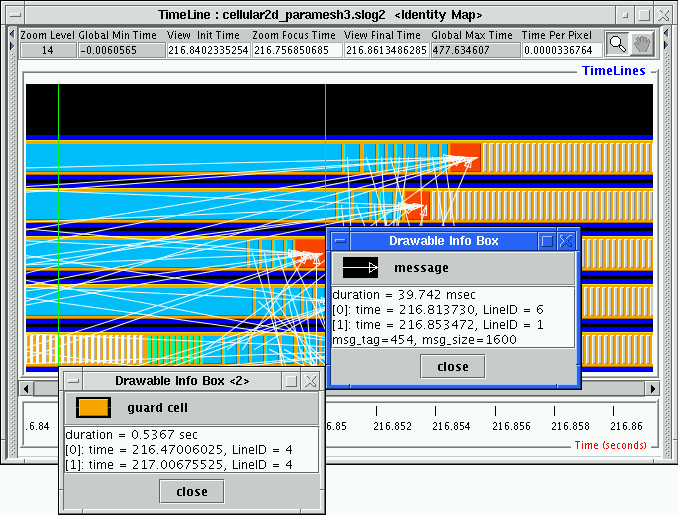
\includegraphics[%
  scale=0.6]{pic/timeline_infobox_real_primitive.png}


\caption{\label{fig:timeline_infobox_real_primitive} Drawable Info Box for
real state and arrow. The Drawable Info Box for the arrow shows the
message size, 1600 byte, and tag ID, 454.}
\end{figure}


Similarly for real drawables, Drawable Info Box can be brought up
by right mouse clicking on the real drawables. In Figure \ref{fig:timeline_infobox_real_primitive},
Drawable Info Boxes for a real arrow and a real state are shown. The
Drawable Info Box for the arrow is invoked by clicking anywhere within
the vicinity of the arrow body%
\footnote{The vicinity width can be adjusted by modifying the parameter CLICK\_RADIUS\_TO\_LINE
in Preference window as listed in Table \ref{table:preference_zoomable_all}.
The default is 3 pixels.%
}, and the info box shows the starttime, start timeline ID, endtime,
and ending timeline ID and some extra information implemented by the
native format. In this example, the message size carried by the specific
arrow is 1600 byte.


\paragraph{Duration Info Box}

%
\begin{figure}[!htbp]
\centering
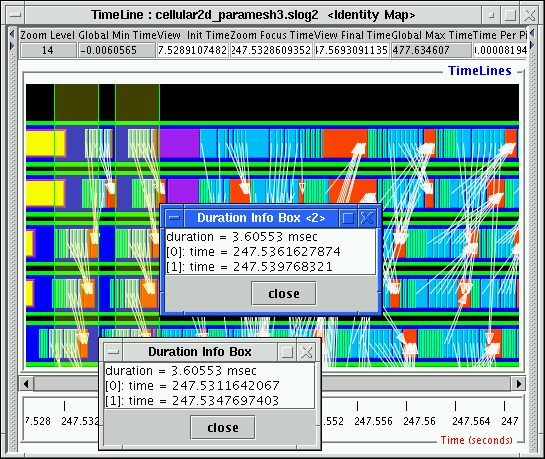
\includegraphics[%
  scale=0.6]{pic/timeline_infobox_duration.png}


\caption{\label{fig:timeline_infobox_duration} Duration Info Box shows the
duration, starttime, and endtime of a time region marked by a pair
of green lines.}
\end{figure}


Duration Info Box is created by right dragging in the timeline canvas
or the time ruler canvas to mark a region in time. The dragged region
will be marked by a pair of green lines and is lightly shaded as well.
Duration Info Box could serve a marker to facilitate the process of
zooming in and out. The information provided by Duration Info Box
could also be used to compare different durations or to measure the
total duration of a collection of subroutine calls. For instance in
Figure \ref{fig:timeline_infobox_duration}, the Duration Info Box
marks all consecutive green states on the fifth timelines. The Duration
Info Box says the total duration of the 9 green states is about 1.74
msec..


\paragraph{Time Info Box}

%
\begin{figure}[!htbp]
\centering
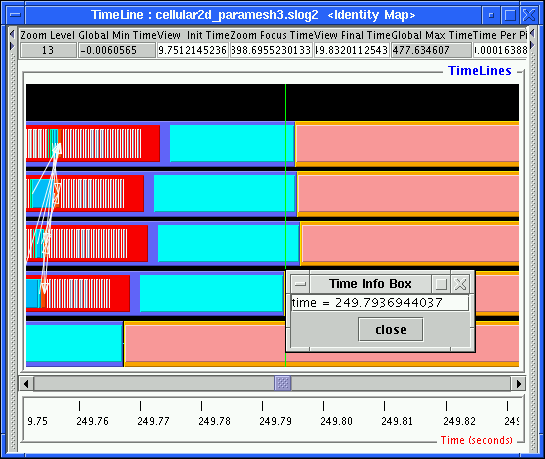
\includegraphics[%
  scale=0.6]{pic/timeline_infobox_time.png}


\caption{\label{fig:timeline_infobox_time} Time Info Box displays the time
of where it pops up.}
\end{figure}


Time Info Box is created by right clicking in the empty space in either
timeline or the time ruler canvas as in Figure \ref{fig:timeline_infobox_time}.
This Info Box is usually used as a marker for a single event in time.


\subsection{Toolbar}

The buttons in the toolbar of Timeline window provides various basic
services to the Timeline window. Table \ref{table:timeline_toolbar}
contains the list of functionalities of the buttons found in the toolbar.

%
\begin{table}[!htbp]
\begin{longtable}{|c|c|c|>{\centering}m{3.5in}|}
\hline 
Icon&
Description&
Shortcut&
Function\tabularnewline
\hline
\hline 

\includegraphics[%
  scale=0.8]{pic/gif2png/Up24.png}&
Up&
Alt-UP&
Scroll upward by half a screen\tabularnewline
\hline 

\includegraphics[%
  scale=0.8]{pic/gif2png/Down24.png}&
Down&
Alt-DOWN&
Scroll downward by half of a screen\tabularnewline
\hline 

\includegraphics[%
  scale=0.8]{pic/gif2png/Edit24.png}&
LabelMark&
none&
Mark the timeline(s)\tabularnewline
\hline 

\includegraphics[%
  scale=0.8]{pic/gif2png/Paste24.png}&
LabelMove&
none&
Move the marked timeline(s)\tabularnewline
\hline 
\includegraphics[%
  scale=0.8]{pic/gif2png/Delete24.png}&
LabelDelete&
none&
Delete the marked timeline(s)\tabularnewline
\hline 
\includegraphics[%
  scale=0.8]{pic/gif2png/TreeExpand24.png}&
LabelExpand&
Alt-E&
Expand the Y-axis tree label by 1 level\tabularnewline
\hline 
\includegraphics[%
  scale=0.8]{pic/gif2png/TreeCollapse24.png}&
LabelCollapse&
Alt-C&
Collapse the Y-axis tree label by 1 level\tabularnewline
\hline 
\includegraphics[%
  scale=0.8]{pic/gif2png/Backward24.png}&
Backward&
Alt-LEFT&
Scroll Backward by half a screen\tabularnewline
\hline 
\includegraphics[%
  scale=0.8]{pic/gif2png/Forward24.png}&
Forward&
Alt-RIGHT&
Scroll Forward by half a screen\tabularnewline
\hline 
\includegraphics[%
  scale=0.8]{pic/gif2png/WinUndo.png}&
ZoomUndo&
Alt-U&
Undo the previous zoom operation\tabularnewline
\hline 
\includegraphics[%
  scale=0.8]{pic/gif2png/ZoomOut24.png}&
ZoomOut&
Alt-O&
Zoom Out by 1 level in time\tabularnewline
\hline 
\includegraphics[%
  scale=0.8]{pic/gif2png/Home24.png}&
ZoomHome&
Alt-H&
Reset zoom to the initial resolution in time\tabularnewline
\hline 
\includegraphics[%
  scale=0.8]{pic/gif2png/ZoomIn24.png}&
ZoomIn&
Alt-I&
Zoom In by 1 level in time\tabularnewline
\hline 
\includegraphics[%
  scale=0.8]{pic/gif2png/WinRedo.png}&
ZoomRedo&
Alt-R&
Redo the previous zoom operation\tabularnewline
\hline 
\includegraphics[%
  scale=0.8]{pic/gif2png/FindBack24.png}&
SearchBackward&
Alt-B&
Search backward in time\tabularnewline
\hline 
\includegraphics[%
  scale=0.8]{pic/gif2png/Find24.png}&
SeachInitialize&
Alt-S&
Search Initialization from last popup InfoBox's time\tabularnewline
\hline 
\includegraphics[%
  scale=0.8]{pic/gif2png/FindFore24.png}&
SearchForward&
Alt-F&
Search forward in time\tabularnewline
\hline 
\includegraphics[%
  scale=0.8]{pic/gif2png/Refresh24.png}&
CanvasReDraw&
Alt-D&
Redraw canvas to synchronize changes from Preference/Legend window
or Y-axis label panel.\tabularnewline
\hline 
\includegraphics[%
  scale=0.8]{pic/gif2png/Print24.png}&
Print&
none&
Print the Timeline window\tabularnewline
\hline 
\includegraphics[%
  scale=0.8]{pic/gif2png/Stop24.png}&
Exit&
none&
Exit the Timeline window\tabularnewline
\hline
\end{longtable}


\caption{\label{table:timeline_toolbar} Table of toolbar's functionalities.}
\end{table}



\subsection{Y-axis Label Panel}

The concealable left panel in Timeline window is called Y-axis label
panel which contains a tree-like representation for Y-axis label for
the timelines. For a SLOG-2 file convertible from CLOG or RLOG with
the default viewmap, the typical Y axis label panel looks like that
is shown in Figure \ref{fig:yaxis_label_panel}. Together with toolbar's
label buttons, e.g. LabelMark and LabelMove, and standard mouse selection
methods listed in Table \ref{table:selection_rules}, labels can be
rearranged easily to create a more easily understood timeline canvas.
For multiple viewmaps SLOG-2 file from IBM's UTE trace environment,
LabelExpand and LabelCollapse buttons will come in handy to expand
and collapse the label tree by one whole level. In order to minimize
unnecessary redraw of the timeline canvas, the synchronization between
the label panel and the timeline canvas is carried out passively,
i.e. user needs to press the CanvasReDraw button in the toolbar to
update the Timeline window with the changes from the label panel.

%
\begin{figure}[!htbp]
\centering
\includegraphics[%
  scale=0.6]{pic/yaxis_label_panel_simple.png}~~~~~~~~~~~~~~~\includegraphics[%
  scale=0.6]{pic/yaxis_label_panel_expanded.png}


\caption{\label{fig:yaxis_label_panel} A simple 1 level Y-axis label tree.
The blue highlighted labels are those that have been selected. The
pulldown menu at the top of panel indicates the value in PREVIEW\_STATE\_DISPLAY
in Preference window}
\end{figure}



\subsection{Row Adjustment Panel}

The concealable right panel in Timeline window contains the row adjustment
panel which is used to determine the row adjustment scheme. There
are 2 different modes in row adjustment panel: row count mode and
row height mode. These 2 modes can be selected by the pulldown menu
at the top of the panel. The row count mode attempts to keep the number
of timelines constant as indicated in the Row Count text field when
the Timeline window resizes. On the other hand, the row height mode
fixes the height of each timeline as indicated by the Row Height text
field. Currently, the height of the timeline can be adjusted up to
the height of the timeline canvas, in that case the Row Count text
field shows a number 1%
\footnote{If the slog2 file contains numerous timelines, increasing the Row
Height will increase the size of the images managed by Jumpshot-4.
This may cause the Java Virtual Machine to exhaust all its memory
if the virtual machine is not set to have enough memory when Jumpshot-4
is started or there isn't enough physical memory in machine that Jumpshot-4
runs on. %
}. The maximum number of timelines that can be displayed is set to
the total number of rows represented by the whole Y-axis label tree%
\footnote{Hence the row height cannot be adjusted all the way to zero.%
}. For multiple viewmaps slog2 file, the Y-axis label tree can be expanded
or collapsed. This could change the maximum number of rows in the
row count slider after user hits the CanvasReDraw button. Coupling
with window resize, the row adjustment panel allows user to magnify
or shrink the height of the timeline as one desires.

%
\begin{figure}[!htbp]
\centering
\subfigure[Row Count mode]{\includegraphics[%
  scale=0.6]{pic/adj_row_count.png}}~~~~~~~~~~~~~~~\subfigure[Row Height mode]{\includegraphics[%
  scale=0.6]{pic/adj_row_height.png}}


\caption{\label{fig:row_adjustment_panel} Row Adjustment Panel determines
the Timeline window's resize scheme. When one of the mode sliders
or text fields is adjusted, the other 3 components will be adjusted
simultaneously.}
\end{figure}



\section{Histogram \emph{Zoomable} Window}

%
\begin{figure}[!htbp]
\centering
\includegraphics[%
  scale=0.5]{pic/histogram_state_all_cumu_excl.png}


\caption{\label{fig:histogram_state_all_cumu_excl}A histogram window of the
whole duration shown in Figure \ref{fig:timeline_popup}.}
\end{figure}


The Histogram window is created through clicking the statistics button
located in the middle of Duration Info Box shown in Figure \ref{fig:timeline_infobox_duration}.
In Figure \ref{fig:histogram_state_all_cumu_excl}, the histogram
window is created for the whole duration of the timeline canvas in
Figure \ref{fig:timeline_popup}, i.e same duration as the complet
slog2 file. In general, the total duration of the histogram canvas
is the same as the duration marked by the Duration Info Box so that
the histogram window functions like a graphical display of statistical
summary of the duration of interest. For instance, it is obvious from
Figure \ref{fig:histogram_state_all_cumu_excl} that the yellow state,
it is MPI\_Barrier in this case, cumulatively takes up the most time.
This is especially true in the last timeline.

Since Histogram window is also a \emph{zoomable} window like Timeline
window, a lot of features like those described in section \ref{sub:Zoomable-and-Scrollable}
for Timeline window are available for Histogram window as well, e.g.
dragged-zoom, grasp and scroll, instant zoom in/out, easy vertical
expansion of timeline, cut and paste of timelines. If some state categories
or timelines need to be made invisible in histogram window, it can
be achieved through disabling the corresponding categories in Legend
window's column V or S or selected corresponding timelines in histogram
window. It is just like that of Timeline window.

Only summary objects can be displayed in the histogram window. Summary
object is similar to preview object discussed earlier. Preview objects
are created during logfile creation stage and cannot be modified during
visualization. Summary objects, on the other hand, are created dynamically
during visualization, i.e. during creation of a Duration Info Box,
so they can be modified easy by end users. There are 2 different kinds
of summary objects: summary state and summary arrow. There is only
1 summary state per timeline and 1 summary arrow for each ordered
pair of timelines%
\footnote{ordered pair of timelines means timeline pair (1,2) is different from
pair (2,1).%
}. Currently 3 different views are available in Histogram window: \emph{States
Only}, \emph{Arrows Only} and \emph{All}. In \emph{States Only} view,
only summary states are displayed. In \emph{Arrows Only} view, only
summary arrows are displayed. In \emph{All} view, both summary states
and arrows are displayed.


\subsection{Summary States}

%
\begin{figure}[!htbp]
\centering
\includegraphics[%
  scale=0.5]{pic/histogram_state_infobox.png}


\caption{\label{fig:histogram_state_infobox} State Summary Info Boxes of
the Histogram window.}
\end{figure}


Since summary states are created through the statistics of real and
preview states, summary states inherit properties of preview states,
i.e. inclusion and exclusion ratios. Because of this, different representations
of summary state are formed based on the PREVIEW\_STATE\_DISPLAY discussed
earlier in section \ref{sub:Preview-State-Display}. Different representation
of summary state can be selected through SUMMARY\_STATE\_DISPLAY pulldown
menu located at the top of the left panel in the histogram window
or through a similar variable defined in Preference window and in
Table \ref{table:preference_zoomable_histogram}. Figure \ref{fig:histogram_state_all_cumu_excl}
is actually a \emph{CumulativeExclusionRatio} view. Since the most
time consuming timeline is the last one, we will zoom in the last
three timelines and use them to discuss the visual representation
of summary state. Figure \ref{fig:histogram_state_infobox} shows
the last three timelines of Figure \ref{fig:histogram_state_all_cumu_excl}.
Each summary state has a gray bordered box. Right mouse clicking at
the bordered box pops up the Summary Info Box for the whole summary
state. The info box lists the total number of real states it contains
and detailed information of what state categories it contains. In
the figure, the summary info boxes at timeline 15 and 13 show that
the timeline 15 summary state contains about 148006 real states and
the timeline 13 summary state has about 859613 real states, i.e. timeline
13 has 5.8 times the number of real states than that of timeline 15
within the same duration. Each summary state also displays the ratios
of the total duration of each member state category to the duration
of the canvas as colored boxes inside the gray bordered box. Right
clicking at any of the colored boxes will display a summary info box
that indicates the color and name of category and the corresponding
ratio for the duration as the highlighted summary info box in the
Figure \ref{fig:histogram_state_infobox}.The remaining duration at
the end of each timeline is unaccounted for. In this particular logfile,
remaining time could be thought of being used for computation.

%
\begin{figure}[!htbp]
\centering
\includegraphics[%
  scale=0.5]{pic/histogram_state_over_incl.png}


\caption{\label{fig:histogram_state_over_incl}The \emph{OverlapInclusionRatio}
view of Figure \ref{fig:histogram_state_infobox}.}
\end{figure}


Switching the SUMMARY\_STATE\_DISPLAY pulldown menu in histogram window
in the figure to \emph{OverlapInclusionRatio} redraws the histogram
canvas. The histogram canvas now looks like one shown in Figure \ref{fig:histogram_state_over_incl}.
Since the sum of all inclusion ratios is greater than 1.0, \emph{CumulativeInclusionRatio}
view is not provided in the histogram window%
\footnote{The view cannot be drawn within same duration as marked in the timeline
window.%
}. All the member categories of the summary states in \emph{OverlapInclusionRatio}
view are drawn from the beginning of the histogram canvas and they
are nested one inside others in decreasing inclusion ratio order,
so the largest inclusion ratios are easily noticeable. In order to
see the smallest ratios, one needs to zoom in around the beginning
of the canvas. In Figure \ref{fig:histogram_state_over_incl}, the
largest inclusion ratios in the 3 visible timelines are all royal
blue and take up about the same amount of time. The 2nd largest ratios
are all orange colored and is smallest in the timeline 15. Therefore
\emph{OverlapInclusionRatio} is good for comparison of member category
contribution among different timelines.


\subsection{Summary Arrows}

%
\begin{figure}[!htbp]
\centering
\includegraphics[%
  scale=0.5]{pic/histogram_arrow.png}


\caption{\label{fig:histogram_arrow} The \emph{Arrows Only} view of the Figure
\ref{fig:histogram_state_all_cumu_excl}.}
\end{figure}


Figure \ref{fig:histogram_arrow} is the \emph{Arrows Only} view of
the histogram window shown in Figure \ref{fig:histogram_state_all_cumu_excl}.
There is a summary arrow per ordered pair of timelines. The duration
of each summary arrow is the total duration of all real arrows taking
place between the ordered pair of timelines within the duration of
the canvas. Notice that it is possible the duration of summary arrow
is longer than that of the canvas. 

%
\begin{figure}[!htbp]
\centering
\includegraphics[%
  scale=0.5]{/home/chan/slog2/slog2sdk_2b/doc/jumpshot-4/tex/pic/histogram_arrow_infobox.png}


\caption{\label{fig:histogram_arrow_infobox} Arrow Summary Info Box of Figure
\ref{fig:histogram_arrow}.}
\end{figure}


Right mouse clicking at the summary arrow will display a Summary Info
Box for the arrow as in the Figure \ref{fig:histogram_arrow_infobox}.
The info box lists the total number of real arrows and the ratio of
the total duration of all real arrows to the duration of canvas. Together
with the info box, summary arrow provides a way to tell which ordered
pair of timelines communicates the most.


\section{Preference Window}

%
\begin{figure}[!htbp]
\centering
\includegraphics[%
  scale=0.6]{pic/preference_pview_state.png}


\caption{\label{fig:preference_pview_state} The Preference window that shows
PREVIEW\_STATE\_DISPLAY}
\end{figure}


As shown in Figure \ref{fig:preference_pview_state} is the Preference
window that adjusts the various display properties of the visualization
program. A list of all the parameters and their definitions are listed
in Tables \ref{table:preference_zoomable_reinit},\ref{table:preference_zoomable_all},
\ref{table:preference_zoomable_timeline}, \ref{table:preference_zoomable_histogram}
and \ref{table:preference_legend}.

%
\begin{table}[!htbp]
\centering
\begin{longtable}{|l|>{\centering}p{1.1in}|p{3.5in}|}
\hline 
Parameter&
Values&
Description\tabularnewline
\hline
\hline 
{\small Y\_AXIS\_ROOT\_LABEL}&
any text&
Label for the root node of the Y-axis tree label in the left panel.\tabularnewline
\hline 
INIT\_SLOG2\_LEVEL\_READ&
+ve integer&
The number of slog2 levels being read into memory when the Timeline
window is initialized, the integer affects the zooming and scrolling
performance exponentially (in a asymptotic sense).\tabularnewline
\hline 
AUTO\_WINDOWS\_LOCATION&
true, false&
Whether to let Jumpshot-4 automatically set windows placement\tabularnewline
\hline 
SCREEN\_HEIGHT\_RATIO&
0.0 ... 1.0&
Ratio of the initial timeline canvas height to the screen height\tabularnewline
\hline 
TIME\_SCROLL\_UNIT\_RATIO&
0.0 ... 1.0&
Unit increment of the horizontal scrollbar in the fraction of timeline
canvas's width.\tabularnewline
\hline
\end{longtable}


\caption{\label{table:preference_zoomable_reinit}Parameters for the section
of \emph{Zoomable Window Reinitialization} in Preference window.}
\end{table}


%
\begin{table}[!htbp]
\centering
\begin{longtable}{|l|>{\centering}p{1.1in}|p{3.5in}|}
\hline 
Parameter&
Values&
Description\tabularnewline
\hline
\hline 
Y\_AXIS\_ROOT\_VISIBLE&
true, false&
Whether to show the top of the Y-axis tree-styled directory label.\tabularnewline
\hline 
ACTIVE\_REFRESH&
false&
Whether to let Jumpshot-4 actively update the timeline canvas.\tabularnewline
\hline 
BACKGROUND\_COLOR&
Black, DarkGray, Gray, LightGray, White&
Background color of the timeline canvas\tabularnewline
\hline 
STATE\_HEIGHT\_FACTOR&
0.0 ... 1.0&
Ratio of the outermost rectangle height to row height. The larger
the factor is, the larger the outermost rectangle will be with respect
to the row height.\tabularnewline
\hline 
NESTING\_HEIGHT\_FACTOR&
0.0 ... 1.0 &
The gap ratio between successive nesting rectangles. The larger the
factor is, the smaller the gap will be.\tabularnewline
\hline 
ARROW\_ANTIALIASING&
default, on, off&
Whether to draw arrow with anti-aliasing lines. Turning this on will
slow down the canvas drawing by a factor of 3.\tabularnewline
\hline 
MIN\_WIDTH\_TO\_DRAG&
integer&
Minimum width in pixel to be considered a dragged operation.\tabularnewline
\hline 
CLICK\_RADIUS\_TO\_LINE&
+ve integer&
Radius in pixel for a click to be considered on the arrow.\tabularnewline
\hline 
LEFTCLICK\_INSTANT\_ZOOM&
true, false&
Whether to zoom in immediately after left mouse click on canvas.\tabularnewline
\hline
\end{longtable}


\caption{\label{table:preference_zoomable_all} Parameters for the section
of \emph{All Zoomable Windows} in Preference window. }
\end{table}


%
\begin{table}[!htbp]
\centering
\begin{longtable}{|l|>{\centering}p{1.9in}|p{2.7in}|}
\hline 
Parameter&
Values&
Description\tabularnewline
\hline
\hline 
STATE\_BORDER&
ColorRaised, ColorLowered, WhiteRaised, WhiteLowered, WhitePlain,
Empty&
Border style of real states.\tabularnewline
\hline 
ARROW\_HEAD\_LENGTH&
+ve integer&
Length of arrow head in pixel.\tabularnewline
\hline 
ARROW\_HEAD\_HALF\_WIDTH&
+ve integer&
Half width of arrow head's base in pixel.\tabularnewline
\hline 
PREVIEW\_STATE\_DISPLAY&
FitMostLegends, OverlapInclusionRatio, CumulativeInclusionRatio, OverlapExclusionRatio,
CumulativeExclusionRatio, BaseAlignedCumulativeExclusionRatio&
Display option of Preview state when Timeline window starts up.\tabularnewline
\hline 
PREVIEW\_STATE\_BORDER&
ColorRaised, ColorLowered, ColorXOR, WhiteRaised, WhiteLowered, WhitePlain,
Empty&
Border style of Preview state.\tabularnewline
\hline 
PREVIEW\_STATE\_BORDER\_W&
integer&
The empty border insets' width in pixel for the Preview state.\tabularnewline
\hline 
PREVIEW\_STATE\_BORDER\_H&
integer&
The empty border insets' height in pixel for the Preview state.\tabularnewline
\hline 
PREVIEW\_STATE\_LEGEND\_H&
integer&
Minimum height of the legend division(category strip) in pixel inside
THICKNESS the Preview state\tabularnewline
\hline 
PREVIEW\_ARROW\_LOG\_BASE&
integer&
The logarithmic base of the number of real arrows amalgamated in Preview
arrow. Hence, this determines the Preview arrow's thickness.\tabularnewline
\hline 
SEARCH\_ARROW\_LENGTH&
integer&
Length of the search marker's arrow in pixel\tabularnewline
\hline 
SEARCH\_FRAME\_THICKNESS&
integer&
Thickness in pixel of the popup frame that highlights the searched
drawable\tabularnewline
\hline 
SEARCHED\_OBJECT\_ON\_TOP&
true, false&
Whether to display the searched object on top of the search frame.\tabularnewline
\hline
\end{longtable}


\caption{\label{table:preference_zoomable_timeline}Parameters for the section
of \emph{Timeline Zoomable Window} in Preference window.}
\end{table}


%
\begin{table}[!htbp]
\centering
\begin{longtable}{|l|>{\centering}p{1.6in}|p{3in}|}
\hline 
Parameter&
Values&
Description\tabularnewline
\hline
\hline 
HISTOGRAM\_ZERO\_ORIGIN&
true, false&
Whether the time ruler is in duration, i.e. starts with 0.0 seconds.\tabularnewline
\hline 
SUMMARY\_STATE\_BORDER&
ColorRaised, ColorLowered, ColorXOR, WhiteRaised, WhiteLowered, WhitePlain,
Empty&
Border style of Summary state when Histogram window starts up.\tabularnewline
\hline 
SUMMARY\_ARROW\_LOG\_BASE&
integer&
The logarithmic base of the number of real arrows amalgamated in Summary
arrow. Hence, this determines the Summary arrow's thickness.\tabularnewline
\hline
\end{longtable}


\caption{\label{table:preference_zoomable_histogram}Parameters for the section
of \emph{Histogram Zoomable Window} in Preference window.}
\end{table}


%
\begin{table}[!htbp]
\centering
\begin{longtable}{|l|>{\centering}p{1.6in}|p{3in}|}
\hline 
Parameter&
Values&
Description\tabularnewline
\hline
\hline 
LEGEND\_PREVIEW\_ORDER&
true, false&
Whether to arrange the legends with a hidden Preview order.\tabularnewline
\hline 
LEGEND\_TOPOLOGY\_ORDER&
true, false&
Whether to arrange the legends with a hidden Topology order.\tabularnewline
\hline
\end{longtable}


\caption{\label{table:preference_legend}Parameters for the section of \emph{Legend
Window} in Preference window.}
\end{table}



\chapter{Special Features}


\section{Search and Scan Facility}

The Level-of-detail support provided in SLOG-2 and Jumpshot-4 tends
to help locate states which are either longer in time or occur very
frequently. States that are short and occur rarely in a big logfile
are very difficult to locate without any special tool. In Jumpshot-4,
a search and scan facility is provided to facilitate this goal. There
are 3 search criteria: search time, searchable timeline IDs and searchable
categories. 

\begin{enumerate}
\item \emph{Search Time} is the time that search starts. It is marked by
a yellow line called search cursor. There are 2 different ways of
setting the search cursor. When the timeline canvas is in Hand mode
as described in Figure \ref{fig:mouse_hand_mode} of section \ref{sub:Zoomable-and-Scrollable},
left mouse clicking will set the search cursor. The other way can
be done in either Hand or Zoom mode. First popup an information dialog
box of any kind using right mouse clicking, then press the SearchInitialize
button in the toolbar to replace the green line by the yellow search
cursor. When there are more than one information dialog box, the information
dialog box that is shown up last will have its green line used to
initialize the search cursor. When Timeline window first starts up,
the search cursor is set at the starttime of the logfile.
\item \emph{Searchable Timeline IDs} are the timelines that search will
operate on, i.e only states on the marked timelines will be returned
by the search facility. These marked timelines can be selected by
clicking on their timeline IDs on Y-axis label panel with rules described
in Table \ref{table:selection_rules}. When nothing is selected, all
timelines are searchable.
\item \emph{Searchable Categories} are categories that have their searchable
checkboxes enabled as in Figure \ref{fig:legend_checkbox_ops}. Only
drawable with searchable category can be returned by the search facility.
By default, all categories in Legend window are searchable. 
\end{enumerate}
%
\begin{figure}[!htbp]
\centering
\includegraphics[%
  scale=0.5]{pic/timeline_search_preview.png}


\caption{\label{fig:timeline_search_preview} Search of state \emph{eos} in
preview stage. The returned state is a preview state containing state
\emph{eos} as shown in the Search Box and Drawable Info Box.}
\end{figure}


After setting any needed search criteria, the search operation can
be carried out by pressing either the SearchForeward or SearchBackward
buttons shown in Table \ref{table:timeline_toolbar}. As shown in
Figure \ref{fig:timeline_search_preview}, the search facility returns
a searched state which is marked by a transparent %
\footnote{the transparency of the 3D raised box can be made opaque by selecting
the SEARCHED\_OBJECT\_ON\_TOP true.%
}box with a 3D raised border and whose starttime is marked by a yellow
search cursor, an upper and a lower 3D arrowheads. The upper 3D arrow's
color matches that of the returned state. In the figure, since the
returned state is a preview state, so the upper 3D arrow is gray in
color as it is shown in Legend window. Accompanied with the 3D raised
bordered box is a popup Search Box that shows the detailed of the
preview state like the Drawable Info Box in Figure \ref{fig:timeline_infobox_preview_state}.
Since the search in the figure is looking for state \emph{eos}, a
Drawable Info Box is shown to indicate the returned 3D bordered box
does contain category \emph{eos} graphically. In order to locate the
real state \emph{eos}, a dragged zoom is performed around the 3D raised
bordered box and the result is shown in Figure \ref{fig:timeline_search_preview_zoomed}.
In the figure, the real \emph{eos} is located in the middle of the
original 3D bordered box and it is pointed by the Drawable Info Box.

%
\begin{figure}[!htbp]
\centering
\includegraphics[%
  scale=0.5]{pic/timeline_search_preview_zoomed.png}


\caption{\label{fig:timeline_search_preview_zoomed} Dragged zoom the region
around the 3D raised bordered box in Figure \ref{fig:timeline_search_preview}
shows the real state \emph{eos.}}
\end{figure}


In general, when searching on big slog2 file, all preview categories
should be set searchable, otherwise searching for real drawables may
not return anything. Because at lower zoom level, there may not be
any real drawables of the categories of interest, only preview drawable
contains the categories of interest. Also, the search facility is
carried out for the drawables that are in the physical memory. In
some rare occasions, drawables in the memory may have been exhausted
for searching before the end of the logfile has been reached, user
may need to advance the search by scroll forward or backward to read
in more drawables and to restart the search again. For a very big
logfile, the search process of a real state may require repeated operations
of search and dragged zoom before the real state can be found. This
process will be automated in the later version of Jumpshot-4.


\section{Tuning of the Timeline Window}

%
\begin{figure}[!htbp]
\centering
\includegraphics[%
  scale=0.5]{pic/timeline_popup_finer.png}


\caption{\label{fig:timeline_popup_finer} The initial Timeline window with
finer preview resolution.}
\end{figure}


One of the major improvements in the new Jumpshot and SLOG-2 is the
scalability in terms of visualization performance. As shown in Figure
\ref{fig:timeline_popup}, there are 14 bands of preview states covering
the whole canvas in the initial Timeline window. By incrementing the
parameter INIT\_SLOG2\_LEVEL\_READ by 1 in Preference window as in
Table \ref{table:preference_zoomable_reinit}, the initial Timeline
window is redisplayed and is shown in Figure \ref{fig:timeline_popup_finer}.
The new Timeline window has 27 bands of preview states instead of
14. The increase preview resolution does offer a more detailed description
of logfile but at the expense of graphical performance. Because every
increment of INIT\_SLOG2\_LEVEL\_READ will roughly double the number
of drawables to be iterated during every zooming or scrolling%
\footnote{it is true for a binary tree%
}. The biggest demand of graphical performance occurs when the zooming
to the level of only pure real drawables from the lower zoom level.
The value of INIT\_SLOG2\_LEVEL\_READ should be chosen so that Jumpshot
does not appear to be too slow during the zooming to the pure real
drawable level. For a fast graphics system, INIT\_SLOG2\_LEVEL\_READ
should be set higher than the default value 4, e.g. 5, so that more
information is present during each view. Slow graphics system should
set INIT\_SLOG2\_LEVEL\_READ lower, e.g. 3.

Another parameter also significantly affects the graphical performance
is ARROW\_ANTIALIASING in Preference window. Setting the parameters
to ON will force Jumpshot to draw all arrows including preview arrows
with anti-aliasing lines. This proves to be an expensive graphical
operation%
\footnote{A typical timeline canvas with arrows will draw roughly a factor 3
slower with anti-aliasing on. %
}. Except when high quality picture is needed like during screen capture
for picture or when anti-aliasing lines are drawn with graphics hardware
support, it is not recommended to turn on ARROW\_ANTIALIASING. 


\section{Estimation of MPI Communication Overhead}

%
\begin{figure}[!htbp]
\centering
\includegraphics[%
  scale=0.5]{pic/timeline_mpi_overhead.png}


\caption{\label{fig:timeline_mpi_overhead} Graphical MPI overhead profiling
through the use of \emph{BaseAlignedCumulativeExclusionRatio} view
of Timeline window in Figure \ref{fig:timeline_popup}.}
\end{figure}


One of the questions that most MPI application developers always want
to know is the overhead of MPI calls in their programs. Essentially
they would like to know what is the communication overhead in their
parallel programs. New SLOG-2 viewer provides a graphical answer to
this question for most MPI profiling system. In MPE profiling system,
MPI states are alway nested deeper than the user-defined states. Therefore
disabling user-defined states and arrows in \emph{CumulativeExclusionRatio}
mode in the Timeline window still leaves all MPI exclusion ratios
intact without distorted the collective meaning of exclusion ratios.
Figure \ref{fig:timeline_mpi_overhead} shows a \emph{CumulativeExclusionRatio}
view in \emph{BaseAligned} mode which looks like a 2-dimensional projection
of a 3-dimensional histogram for a timeline vs time coordinate system.
The base aligned feature is for easy comparison of preview states'
heights. It becomes apparent from the figure that not only do we know
the yellow state, i.e. MPI\_Barrier, takes up most time in the program,
we also know when and where MPI\_Barrier consumes most time. The combination
of disabling user-defined states and use of \emph{BaseAlignedCumulativeExclusionRatio}
Timeline view provides a powerful and convenient way to estimate MPI
communication overhead. Together with the zoomable capability of the
Timeline window, user can easily zoom in to identify the time and
location of the bottleneck that causes the biggest communication overhead.
For an overall estimate of MPI overhead, a histogram window over the
whole duration of the timeline canvas can be obtained and is shown
in Figure \ref{fig:histogram_mpi_overhead}. The vacuum region in
each timeline is assumed to be used by user computation.

%
\begin{figure}[!htbp]
\centering
\includegraphics[%
  scale=0.5]{pic/histogram_mpi_overhead.png}


\caption{\label{fig:histogram_mpi_overhead} An overall MPI overhead histogram
for Figure \ref{fig:timeline_mpi_overhead}.}
\end{figure}

\end{document}
